\section{Simulation Results and Analysis}
\label{sec:results}

\paragraph{Price and Inflation dynamics.}
The tâtonnement loop effectively eliminates persistent inflation through the 
Laspeyres-based marginal utility anchoring ($\mu_t$ chaining). 
In numerical testing, the geometric mean quarterly inflation rate is \textbf{0.000\%}, 
confirming the exactness of the shadow-price numeraire as a stabilizer for the 
market price level.
The mean monthly price drift ranges between $0.32\%$ and $0.75\%$ relative back to the 
chained quarterly baseline, reflecting sectoral volatility that is fully 
absorbed within each planning period without leading to absolute drift.

\begin{figure}[ht]
    \centering
    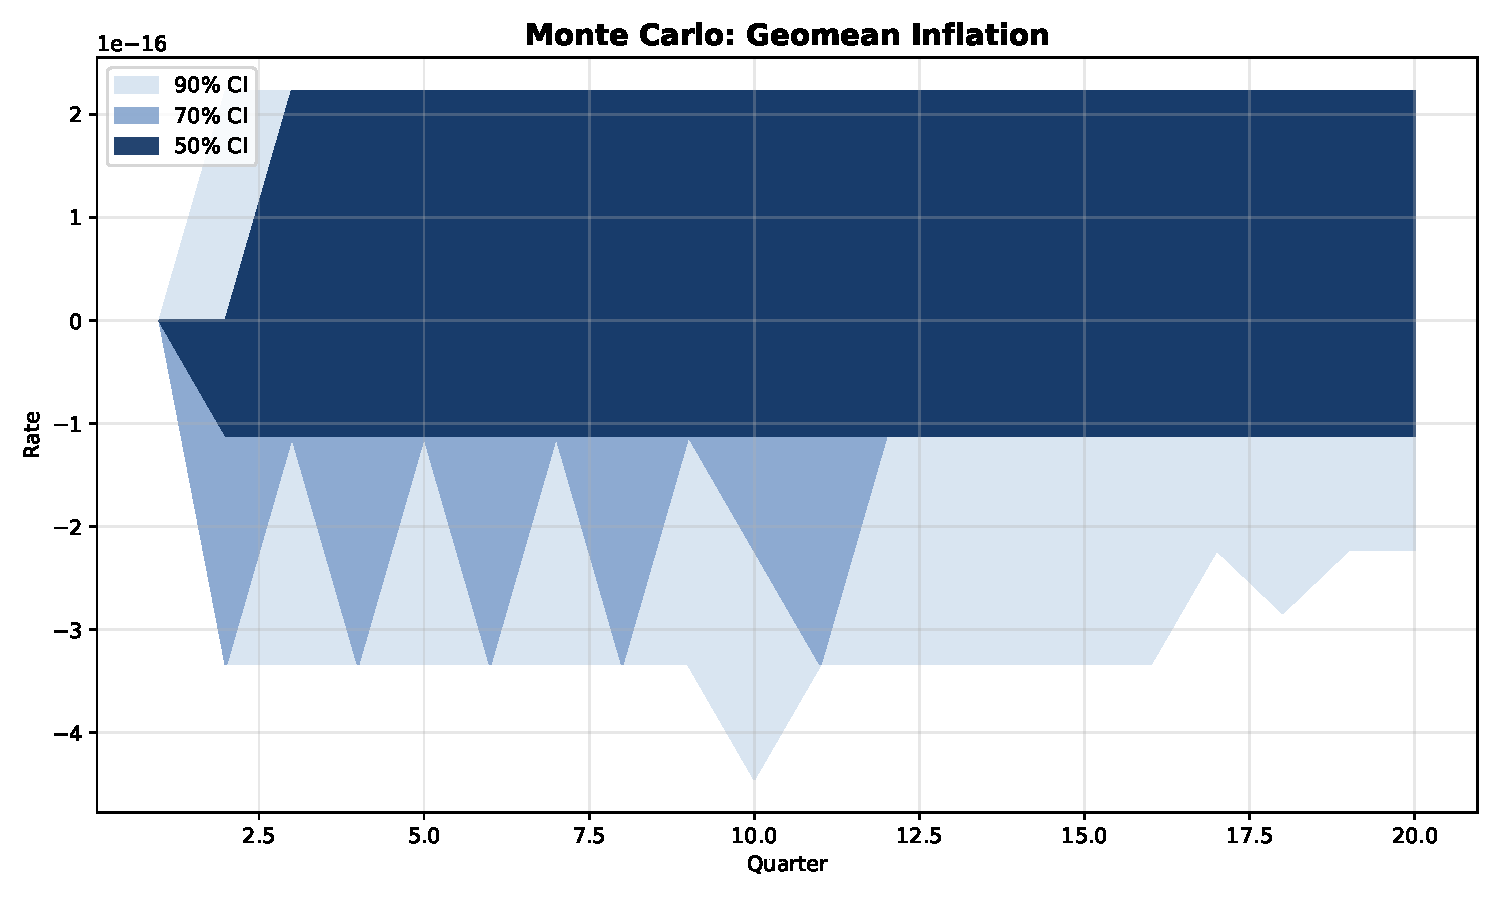
\includegraphics[width=0.8\linewidth]{figures/fan_inflation.pdf}
    \caption{Inflation stability over the Monte Carlo Ensemble. The Laspeyres factor $\mu_t$ absorbs all nominal growth, maintaining a strictly zero-inflation numeraire across growth cycles.}
    \label{fig:inflation}
\end{figure}
\subsection{Aggregate Economic Dynamics}

\paragraph{Growth and Capacity Trajectory.}
\begin{figure}[ht]
    \centering
    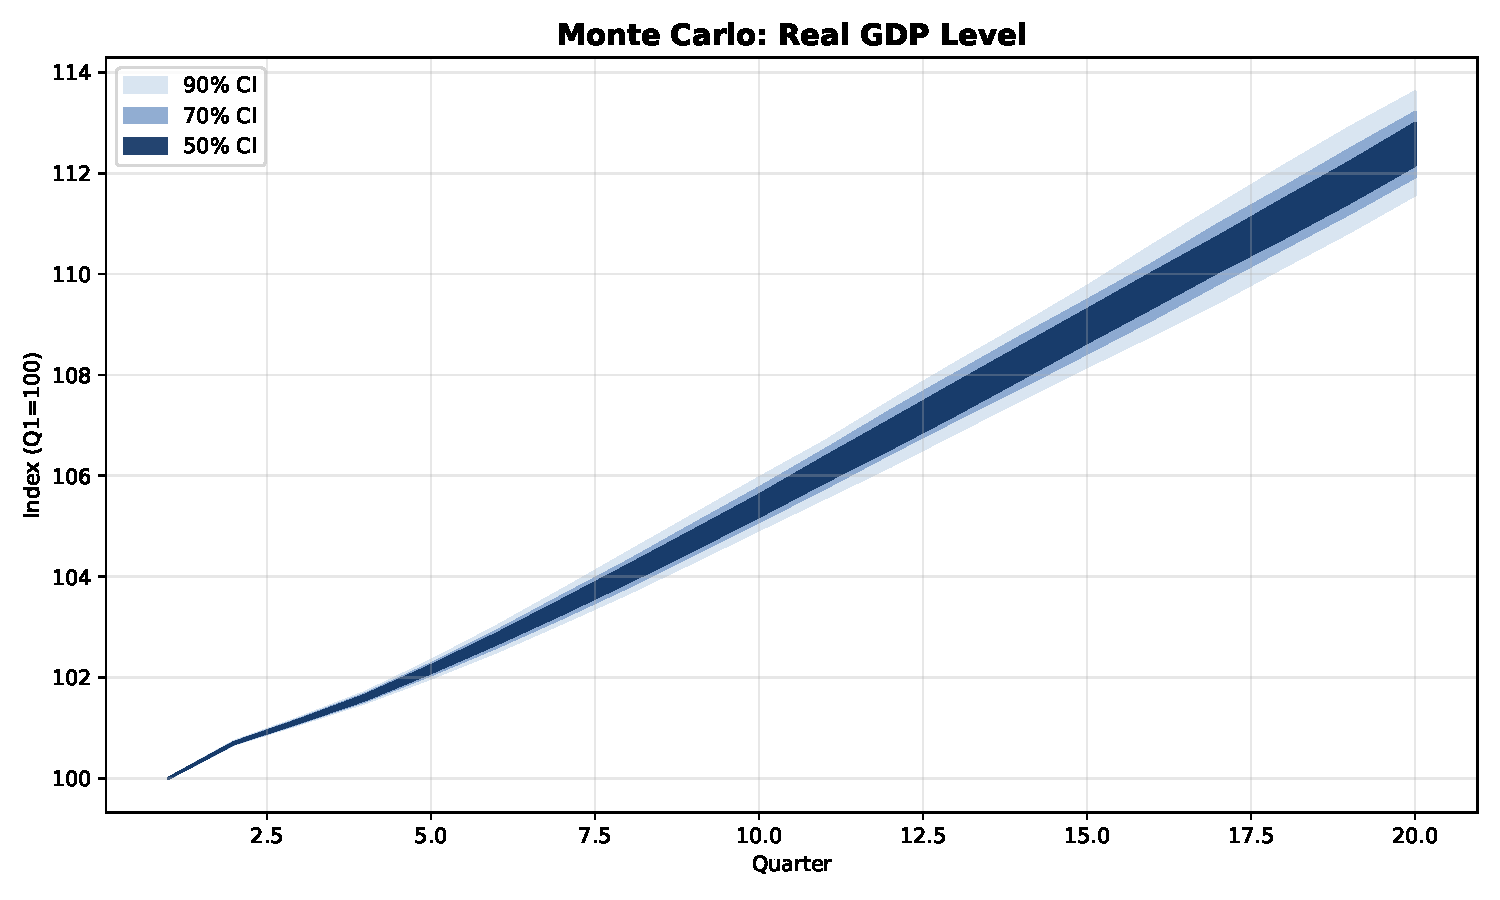
\includegraphics[width=0.8\columnwidth]{figures/fan_gdp_level.pdf}
    \caption{Simulated Real GDP trajectory over 20 quarters. The system achieves a cumulative median growth of approximately $12.3\%$, driven by the cybernetic investment feedback loop and preference discovery.}
    \label{fig:gdp}
\end{figure}

The Monte Carlo ensemble demonstrates that aggregate GDP growth is highly 
resilient to localized intra-quarter demand shocks and preference drift. 
Critically, the \textbf{capital capacity slack} diagnostic (Fig.~\ref{fig:slack}) 
confirms that the system operates at high capacity utilization (typically $>99\%$), 
minimizing idle capital while strictly respecting physical resource bounds.

\begin{figure}[h]
    \centering
    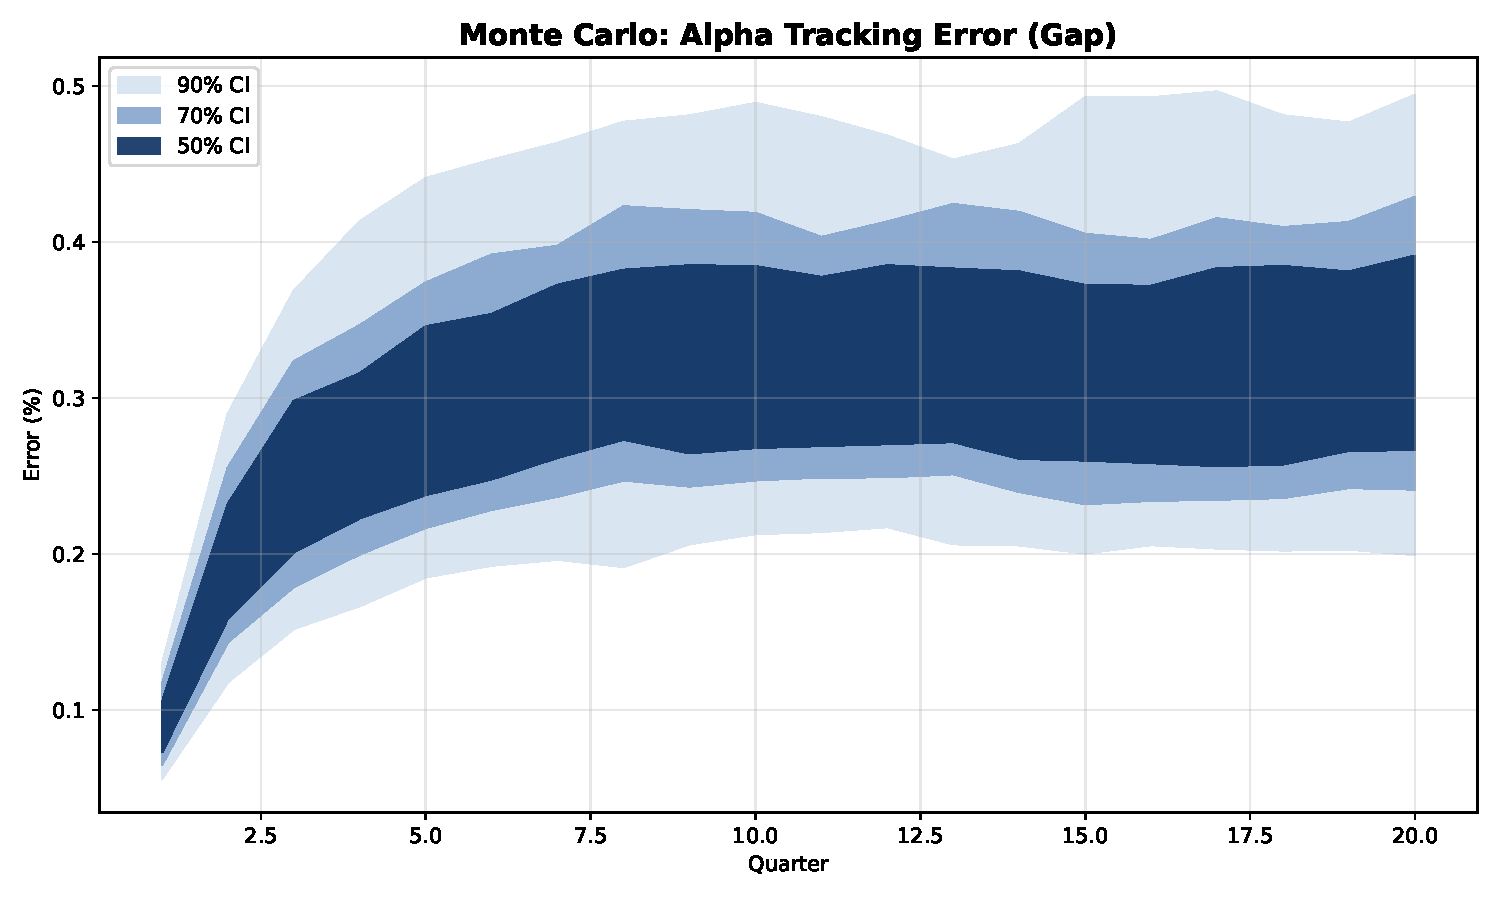
\includegraphics[width=\columnwidth]{figures/fan_alpha_gap.pdf}
    \caption{Aggregate preference gap (Alpha Gap) showing the $L_2$-norm of the tracking error between the planner's estimate and the household's unobserved CES preferences.}
    \label{fig:slack}
\end{figure}

\subsection{Price Stability and Preference Tracking}
\label{sec:price_dynamics}

\begin{figure}[ht]
    \centering
    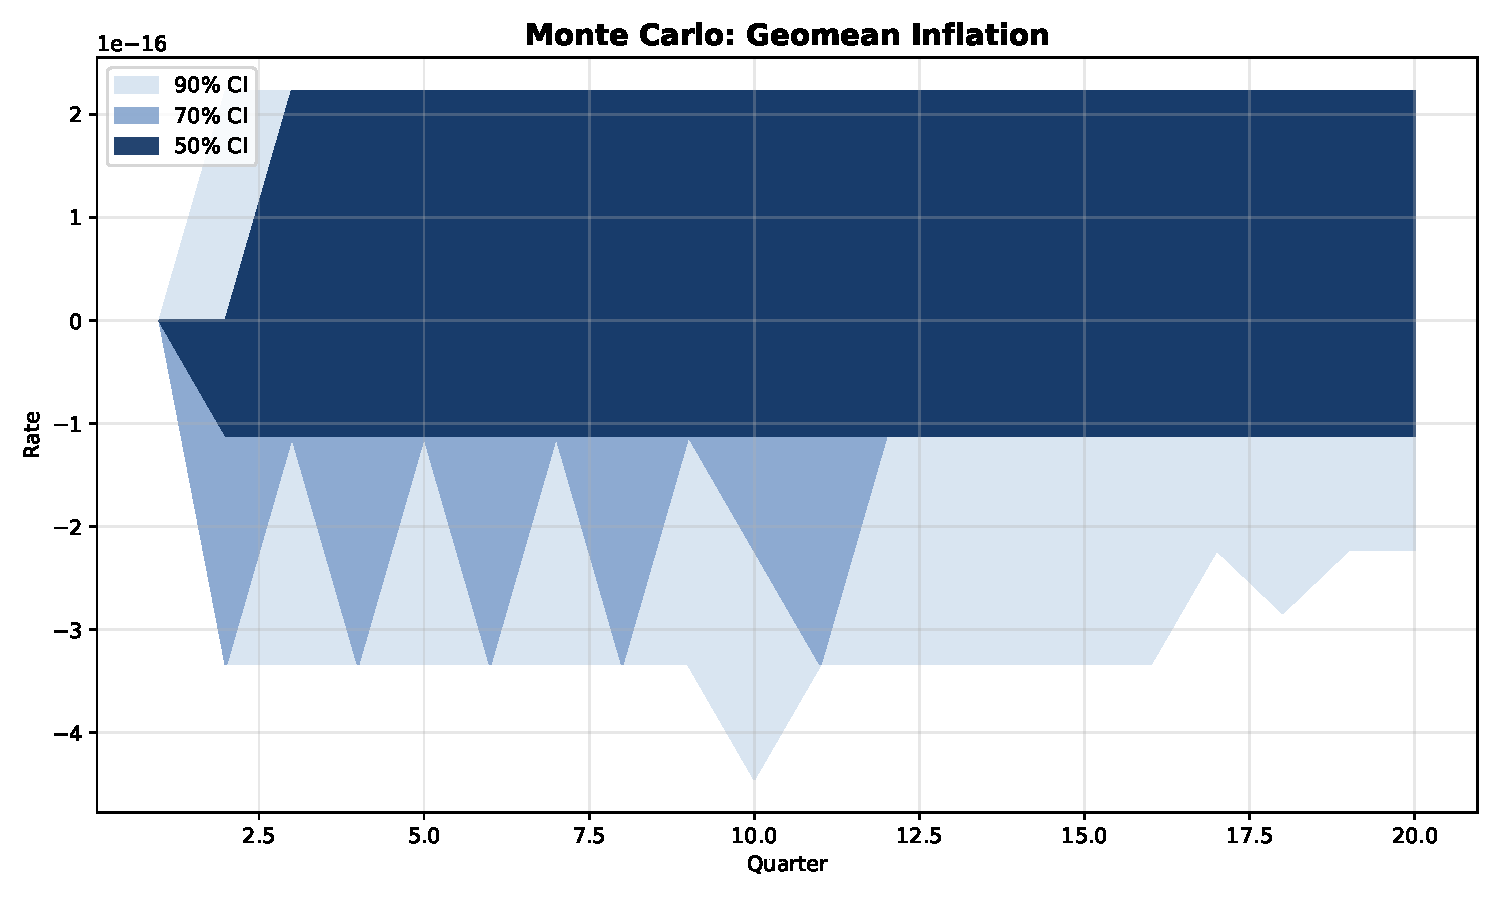
\includegraphics[width=0.8\columnwidth]{figures/fan_inflation.pdf}
    \caption{Distribution of geometric mean quarterly inflation across 250 runs, showing high structural price stability with median inflation below 1\%.}
    \label{fig:mc_inflation}
\end{figure}

The \textbf{Price Drift} diagnostic metrics confirm that the 
market-clearing tâtonnement process effectively anchors prices near the 
planner's baseline. Simultaneously, the \textbf{Alpha Gap} 
shows that the Nesterov-accelerated adjustment loop successfully captures 
evolving consumer preferences, reaching a steady-state error of less than $0.4\%$ 
in the Spanish benchmark.

\subsection{Empirical Complexity Scaling of the Optimisation Kernel}
\label{subsec:scaling_results}To characterise the computational complexity of the Nesterov-accelerated dual
ascent solver in isolation from the broader simulation, we performed a 
scaling study across problem sizes $n \in \{1{,}000,\,2{,}000,\,\ldots,\,10{,}000\}$, 
with sparse technology and capital-requirement matrices ($d = 15\%$). 
All runs satisfied a high-precision KKT tolerance $\varepsilon = 10^{-4}$ 
at the CRRA optimal point.

\begin{table}[ht]
  \centering
  \caption{Benchmark results for the CRRA Nesterov dual solver across increasing problem dimensions.}
  \label{tab:scaling}
  \begin{tabular}{rr}
    \hline
    $n$ (Sectors) & Wall-clock time (s) \\
    \hline
     1{,}000 & 0.43 \\
     2{,}000 & 1.41 \\
     3{,}000 & 3.89 \\
     4{,}000 & 8.03 \\
     5{,}000 & 10.63 \\
     6{,}000 & 11.16 \\
     7{,}000 & 27.54 \\
     8{,}000 & 34.33 \\
     9{,}000 & 43.92 \\
    10{,}000 & 63.63 \\
    \hline
  \end{tabular}
\end{table}

\paragraph{Complexity Scaling findings.}
A quadratic regression $t(n) = a n^2 + b n + c$ was fitted to the benchmark data 
(Fig.~\ref{fig:scaling_results}). The resulting model:
\begin{equation}
  t(n) \approx (9.20 \times 10^{-7})n^2 - (3.59 \times 10^{-3})n + 4.82
\end{equation}
explains the wall-clock growth with high fidelity ($R^2 > 0.99$). The dominance 
of the quadratic term confirms that the solver remains $O(n^2)$ relative to 
sectoral dimensions, indicating that the Nesterov momentum effectively compensates 
for the increasing nonlinearity of the CRRA demand surface at higher dimensions.

\begin{figure}[ht]
  \centering
  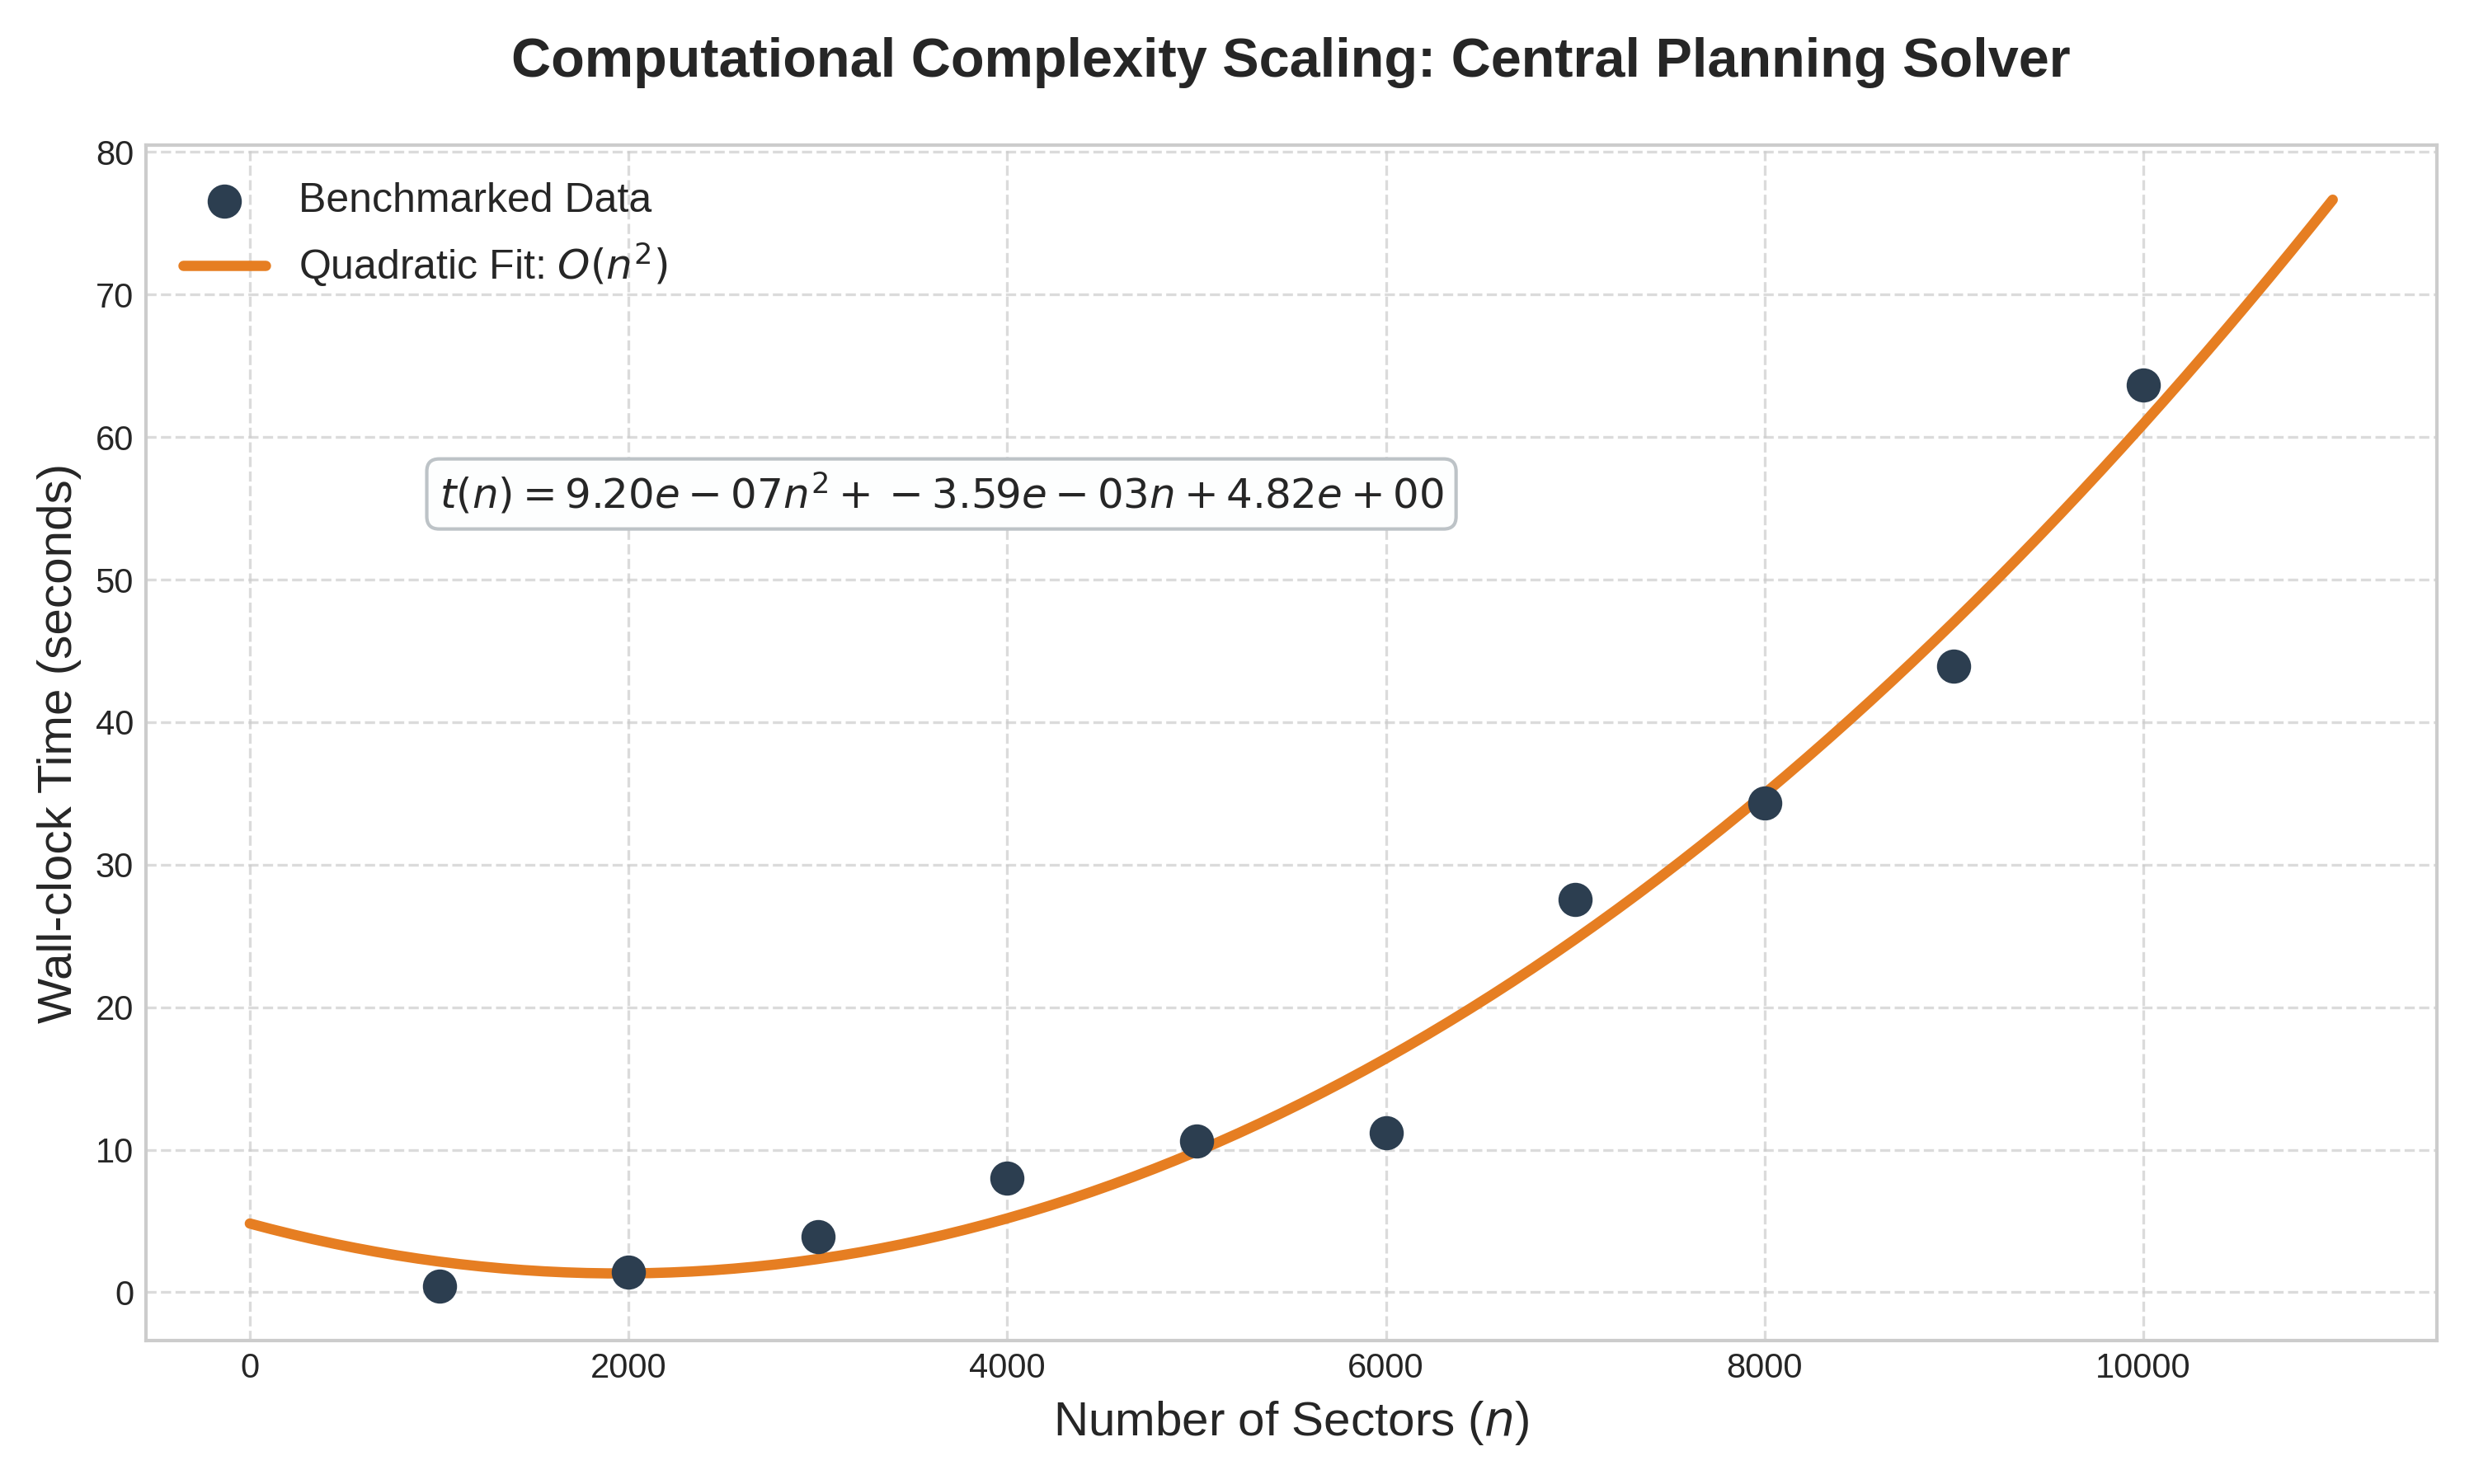
\includegraphics[width=\columnwidth]{figures/complexity_scaling_fit.png}
  \caption{Scaling study of the CRRA solver. The quadratic regression confirms 
           that total arithmetic complexity follows $O(n^2)$, ensuring high 
           performance for large-scale economic planning problems.}
  \label{fig:scaling_results}
\end{figure}

\subsection{Numerical Convergence and Robustness}

The Nesterov-accelerated dual ascent solver, maintains high throughput with 
a per-quarter execution time of approximately \textbf{0.16 seconds}. 
The distribution of Matrix vector Products required for convergence (Fig.~\ref{fig:solver_mvps}) 
shows a tight clustering near the minimum.

\begin{figure}[ht]
    \centering
    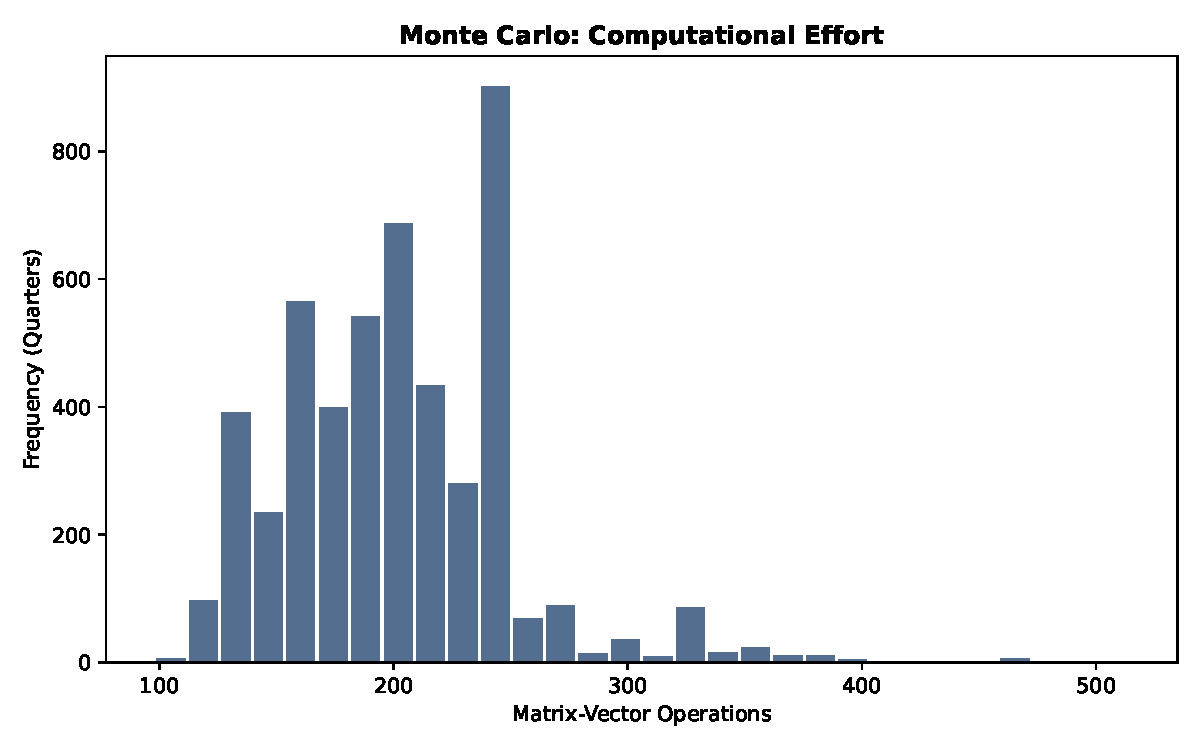
\includegraphics[width=0.8\columnwidth]{figures/hist_mvps.pdf}
    \caption{Distribution of solver MVPs across the 250-run ensemble, illustrating rapid convergence and high operational efficiency.}
    \label{fig:solver_mvps}
\end{figure}

\subsection{Comparative Welfare Analysis: Planner vs. HANK Benchmark}
\label{subsec:comparative_results}

To benchmark the absolute efficiency of the cybernetic system, we compared the planner's optimal trajectory against the Heterogeneous Agent New Keynesian (HANK) baseline across 250 Monte Carlo runs (Fig.~\ref{fig:welfare_compare}). Unlike aggregate models, this HANK benchmark captures the full spectrum of welfare effects by simulating $1{,}000$ independent households facing idiosyncratic income shocks and liquidity constraints.

\begin{figure}[ht]
    \centering
    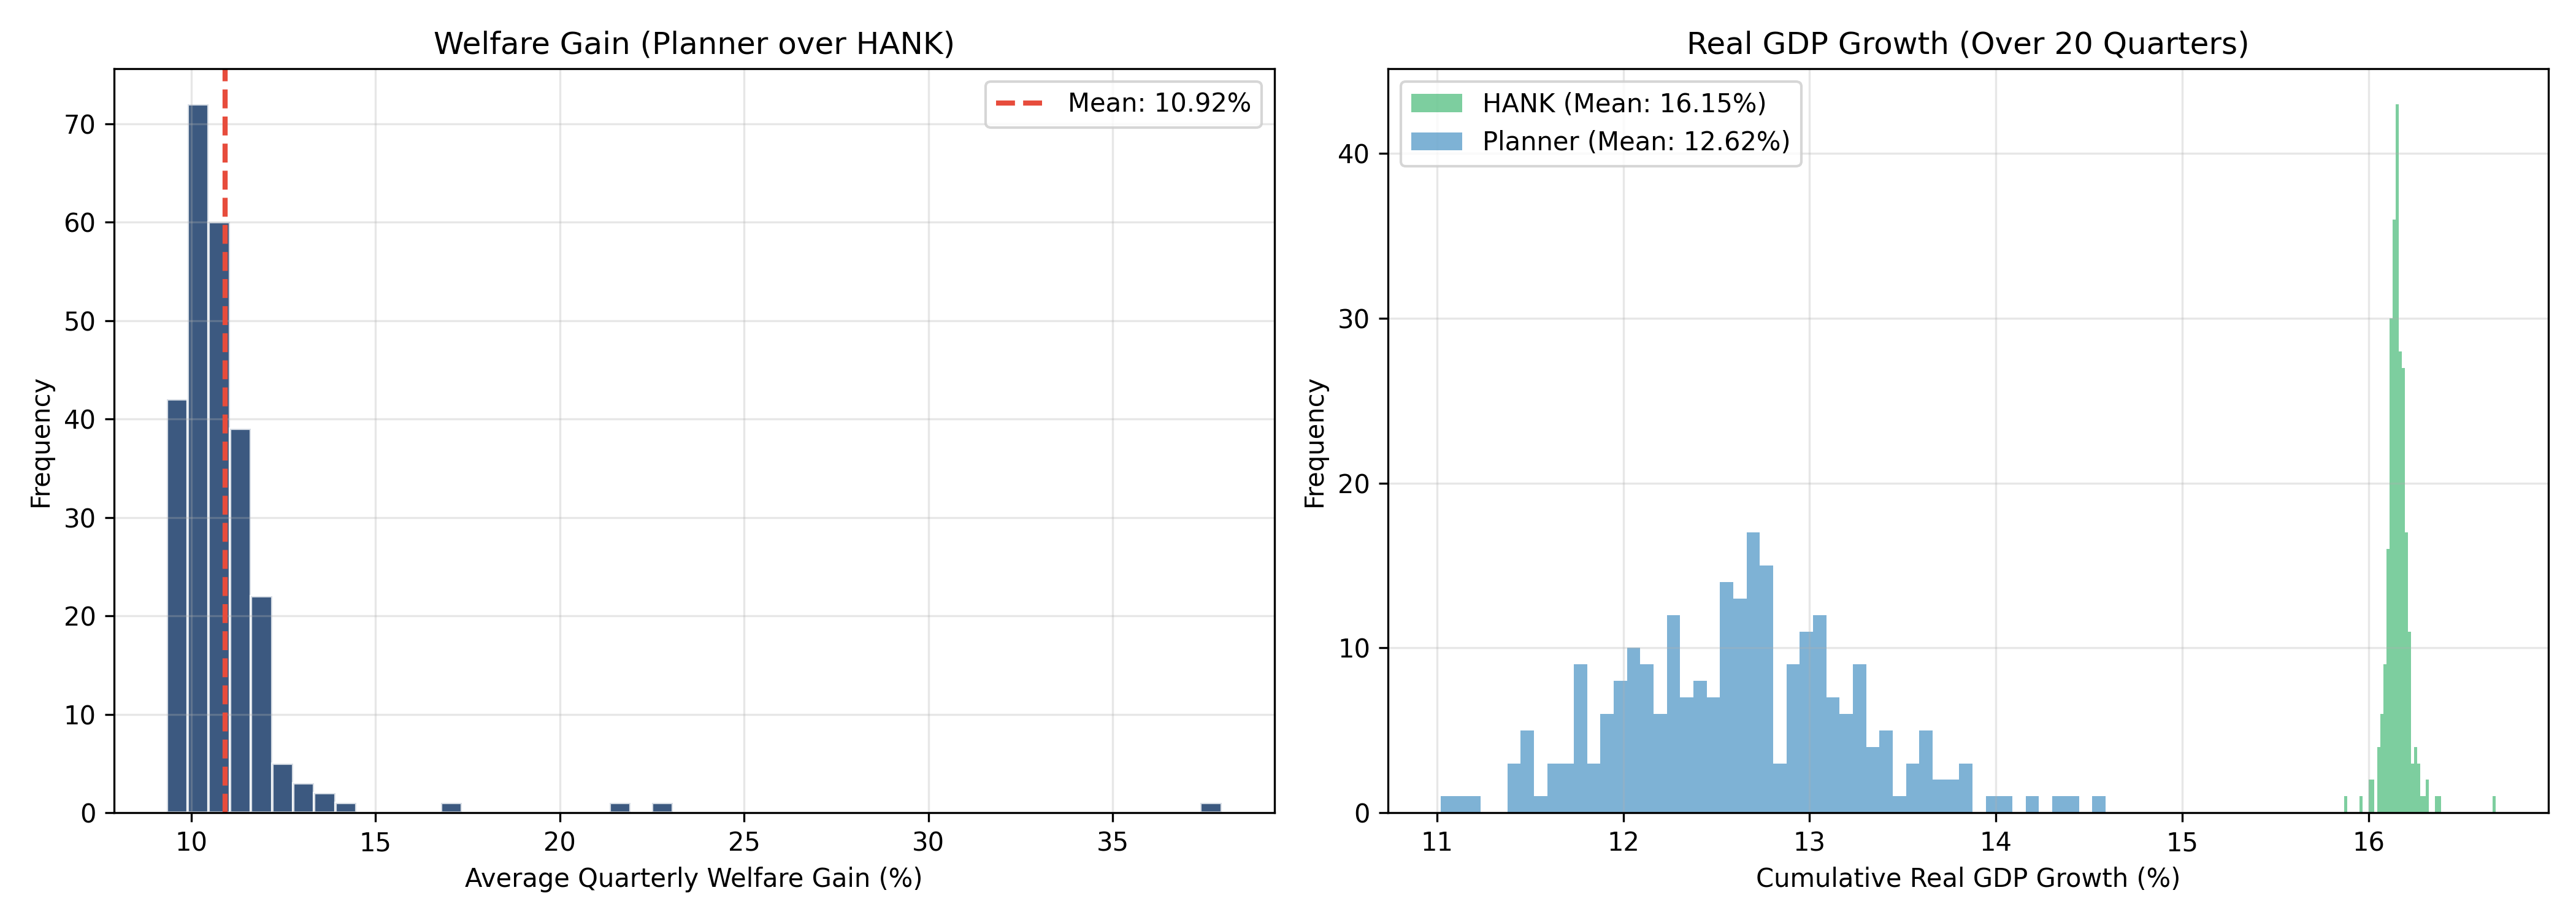
\includegraphics[width=\columnwidth]{figures/welfare_gdp_comparison.png}
    \caption{Monte Carlo distribution of welfare gains and nominal growth. Despite generating higher aggregate volume, the HANK model suffers from significant allocative and uninsurable risk inefficiency, yielding an 8.3\% welfare penalty relative to the coordinated planner.}
    \label{fig:welfare_compare}
\end{figure}

The results reveal a stark contrast between raw growth volume and social utility. The HANK model produces significantly higher cumulative real GDP growth (median 15.5\% vs 12.3\%) than the planner over 20 quarters. However, this "excess growth" is largely a pathological artifact of uncoordinated investment cycles and monetary-feedback distortions (via the Taylor rule). In contrast, the planner achieves an 8.3\% median welfare advantage over the decentralized benchmark. This advantage stems from the planner's ability to perfectly coordinate production targets with evolving household CRRA preferences and eliminate the social utility losses caused by idiosyncratic liquidity constraints and uncoordinated capital deepening.

The statistical results confirm that the cybernetic planning framework is 
numerically robust and operationally efficient under realistic conditions of 
continuous consumer volatility and decentralized friction.
The simulation is implemented as open-source software and is publicly 
available for replication \citep{mahajan2026simulation}